\chapter{Dust Attack}
Gli obiettivi principali di questa tesi sono:
\begin{itemize}
\item Definire il Dust Attack, spiegandone le conseguenze e le possibili contromisure;
    \item Presentare delle statistiche generali su come venga speso il dust, in particolare mostrare se e quanto possa essere efficace un Dust Attack mostrando gli effetti del dust sulla de-anonimizzazione degli address;
    \item Descrivere due pattern interessanti che sono stati trovati e che potrebbero rappresentare casi di Dust Attack.
\end{itemize}
Il Dust Attack è una nota tecnica che sfrutta gli importi dust. È importante quindi spiegare cosa sia il dust e in generale quali possano essere i suoi possibili impieghi.
\section{Dust}
\section{Usi del dust}
\subsection{Satoshi Dice}
Satoshi Dice è un noto "gioco di scommesse basato su blockchain" nato nell'Aprile 2012 \cite{SD}. A differenza dei tradizionali software di gioco online, le scommesse con Satoshi Dice possono essere inviate senza accedere al sito Web né eseguire alcun software client. Per giocare, viene effettuata una transazione Bitcoin a uno degli address resi pubblici da Satoshi Dice, ciascuno con pagamenti diversi. Tutti gli address resi pubblici da Satoshi Dice sono vanity address, tutti gli address infatti presentano il prefisso \textbf{1dice}. Un vanity address in generale è un address Bitcoin con le stesse funzionalità di qualsiasi altro address ma presenta una stringa personalizzata contenente una parola o un messaggio comprensibili alle persone. Un esempio di vanity address è 1BoatSLRHtKNngkdXEeobR76b53LETtpyT, che contiene la parola Boat. Ogni indirizzo \textbf{1dice} presenta probabilità diverse di vincere la scommessa, generalmente minore è la probabilità maggiore è il compenso che si ottiene da una vincita. Per esempio 1dice1e6pdhLzzWQq7yMidf6j8eAg7pkY offre una probabilità dello 0,0015\% di vincere 64 000 volte la puntata originale. Per determinare se una scommessa è vincente o perdente, Satoshi Dice utilizza un metodo per produrre un numero casuale, il quale viene assegnato al giocatore. Il servizio successivamente utilizza una combinazione dell'hash della transazione della scommessa ed esegue un hash SHA2 a 512 bit per quell'hash della transazione utilizzando un segreto sconosciuto al giocatore. I primi quattro byte di quell'hash diventano il numero per determinare il fortunato vincitore.

Il servizio, dopo aver determinato le scommesse vincenti e quelle perdenti, invia una transazione in risposta con il pagamento al vincitore e restituisce un sinoglo satoshi ai giocatori perdenti per comunicare loro la perdita.
\subsection{OP RETURN}
Le transazioni in Bitcoin sono molto più complesse \cite{script} di come descritte nel capitolo precedente \ref{Transazioni}, non contengono solo valori come address e importo ma includono anche del codice, in particolare ogni transazione comprende anche degli script che descrivono come la persona successiva che desidera spendere i bitcoin trasferiti possa accedervi. Bitcoin utilizza un sistema di script Forth-like, basato su stack e non Turing-completo; questa scelta di evitare i loop è intenzionale in quanto impedisce possibili cicli infiniti. Gli script \cite{opcode} in Bitcoin sono:
\begin{itemize}
    \item Senza stato: non esiste uno stato prima dell'esecuzione di uno script né viene salvato dopo l'esecuzione.
    \item Deterministici: uno script viene eseguito alla stessa maniera in ogni sistema.
    \item Semplici e compatti: le istruzioni, gli OP\_CODE, sono codificate in un singolo byte. In totale ci sono 75 istruzioni funzionanti e 15 disabilitate.
\end{itemize}
Gli OP\_CODE in Bitcoin comprendono diverse categorie con alcuni esempi:
\begin{itemize}
    \item aritmetica di base: OP\_ADD, OP\_SUB;
    \item controllo di flusso: OP\_IF, OP\_ELSE;
    \item logica bit a bit: OP\_EQUAL;
    \item gestione stack: OP\_DROP, OP\_SWAP;
    \item hashing: OP\_SHA1, OP\_SHA256;
    \item verifica firma o multifirma: OP\_CHECKMULTISIG.
\end{itemize}

Le transazioni Bitcoin non forniscono un campo dove si possono salvare dati arbitrari \cite{arbdata}. Tuttavia, gli utenti hanno ideato vari modi creativi per codificare i dati nelle transazioni. Questi metodi però modificavano il protocollo di transazione rendendo inspendibili gli output così generati. Il problema è che questi output non erano facilmente distinguibili dagli altri quindi in nodi della rete dovevano salvarli nei loro UTXO set.

L'UTXO(Unspent Transaction Output) set è l'insieme degli output riscattabili di tutte le transazioni della blockchain. Per essere valida, una transazione deve
utilizzare solo elementi dell'UTXO come input.

Poiché questo set, per motivi di efficienza, è solitamente memorizzato nella RAM \cite{utxo} questa pratica influiva negativamente sul consumo di memoria dei nodi \cite{stresstest}.

Per risolvere tale problema nel 2014 è stato reso standard il codice OP\_RETURN \cite{opreturnstandard} . Questo OP\_CODE era presente fin dalla nascita di Bitcoin, però era considerato non-standard proprio perchè la scrittura di dati arbitrati sulla blockchain non viene considerata una buona pratica. Questo codice permette di segnare un output della transazione come non valido, quindi successivamente non potrà essere speso. Siccome gli output con questo OP\_CODE non possono essere spesi, possono essere rimossi dall'UTXO set. In questo modo OP\_RETURN risolve il problema del consumo di memoria spiegato precedentemente. Il limite iniziale per la memorizzazione dei dati con questo codice era pianficato per essere di 80 byte, ma inizialmente ne furono concessi 40(versione 0.9.0).  La versione 0.11.0 \cite{v11} ha esteso il limite di dati a 80 byte e la versione 0.12.0 \cite{v12} fino a un massimo di 83 byte. 
\textbf{SPIEGARE ALCUNI ESEMPI DI OP RETURN}
\section{Dust Attack}
Il dust attack è una nota tecnica, presente nel mondo delle criptovalute, il cui obiettivo è la 
de-anonimizzazione del proprietario di un wallet. L'obiettivo dell'attaccante è di collegare address diversi tra loro, ovvero riuscire a capire quali address appartengano ad uno stesso wallet.\\
La strategia usata dagli attaccanti è quella di inviare a diversi address piccoli importi dust.\\
In Bitcoin, il termine dust si riferisce agli importi inferiori alla fee minima richiesta per spenderli in una transazione. Come specificato in \cite{BtcDev}, un
importo è considerato dust se è inferiore alla soglia di 546 satoshi.\\
Per effettuare il dust attack quindi è necessario avere a disposizione una certa quantità di bitcoin da poter dividere in centinaia, o migliaia, di output dust, come mostrato in figura \ref{fig:Dust_attack}.
L'attaccante invia questi piccoli importi a diversi address confidando che vengano spesi successivamente in una nuova transazione insieme ad altri address. Come spiegato nel capitolo precedente, è raro infatti che gli address di input di una transazione appartengano a più utenti, si presume quindi che tutti gli address appartengano a un solo utente; quindi sono collegati tra loro.
\begin{figure}[h!]
    \centering
    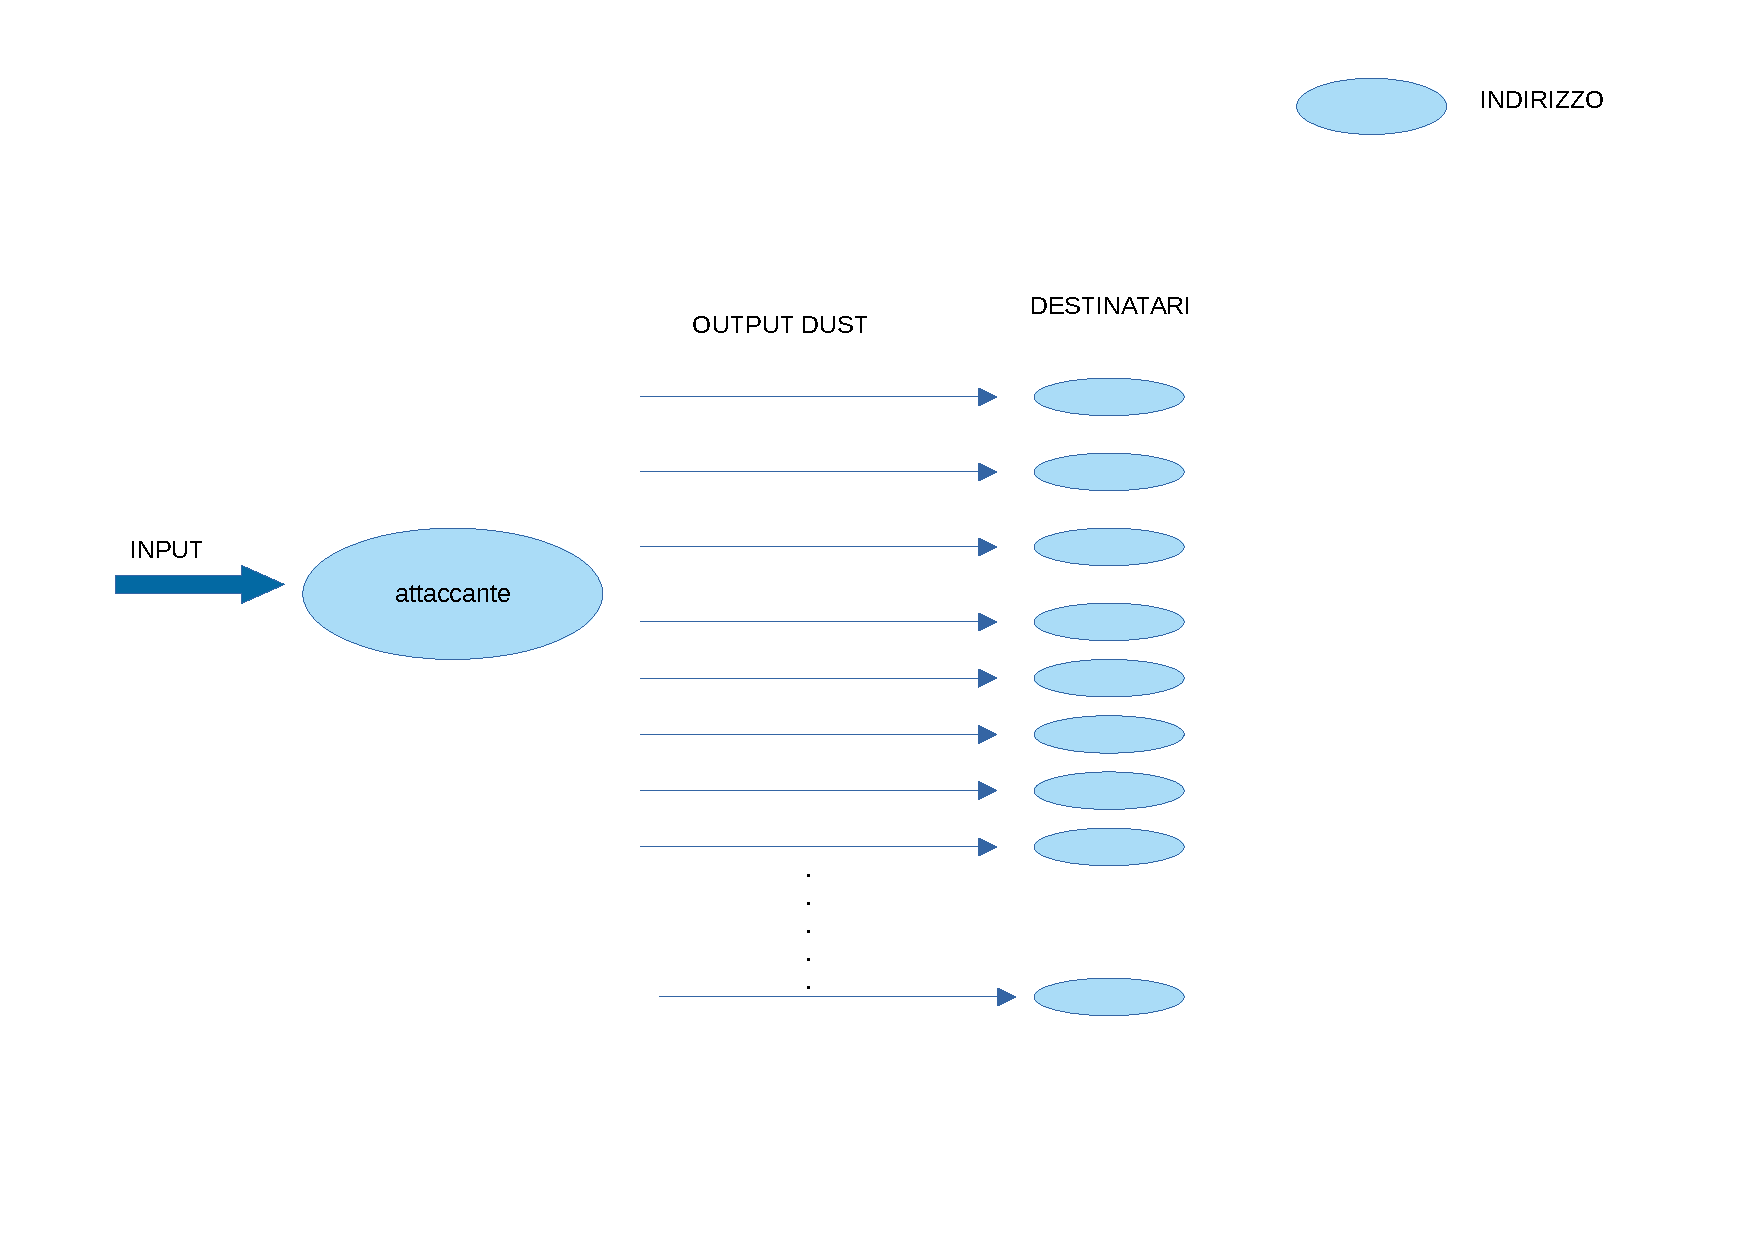
\includegraphics[scale=0.5]{Images/dust_attack.pdf}
    \caption{Schema Dust Attack}
    \label{fig:Dust_attack}
\end{figure}
\FloatBarrier
Una volta effettuato l'attacco possono esserci tre possibili esiti: 
    \begin{enumerate}
        \item attacco di successo;
        \item attacco fallito;
        \item dust bruciato.
    \end{enumerate}
Nel primo caso, mostrato in figura \ref{fig:success}, la vittima genera una transazione in cui spende l'importo dust ricevuto insieme ad almeno un altro dei suoi address. L'attaccante può quindi collegarli e capire che appartengono allo stesso utente.\\\\
\begin{figure}[h!]
    \centering
    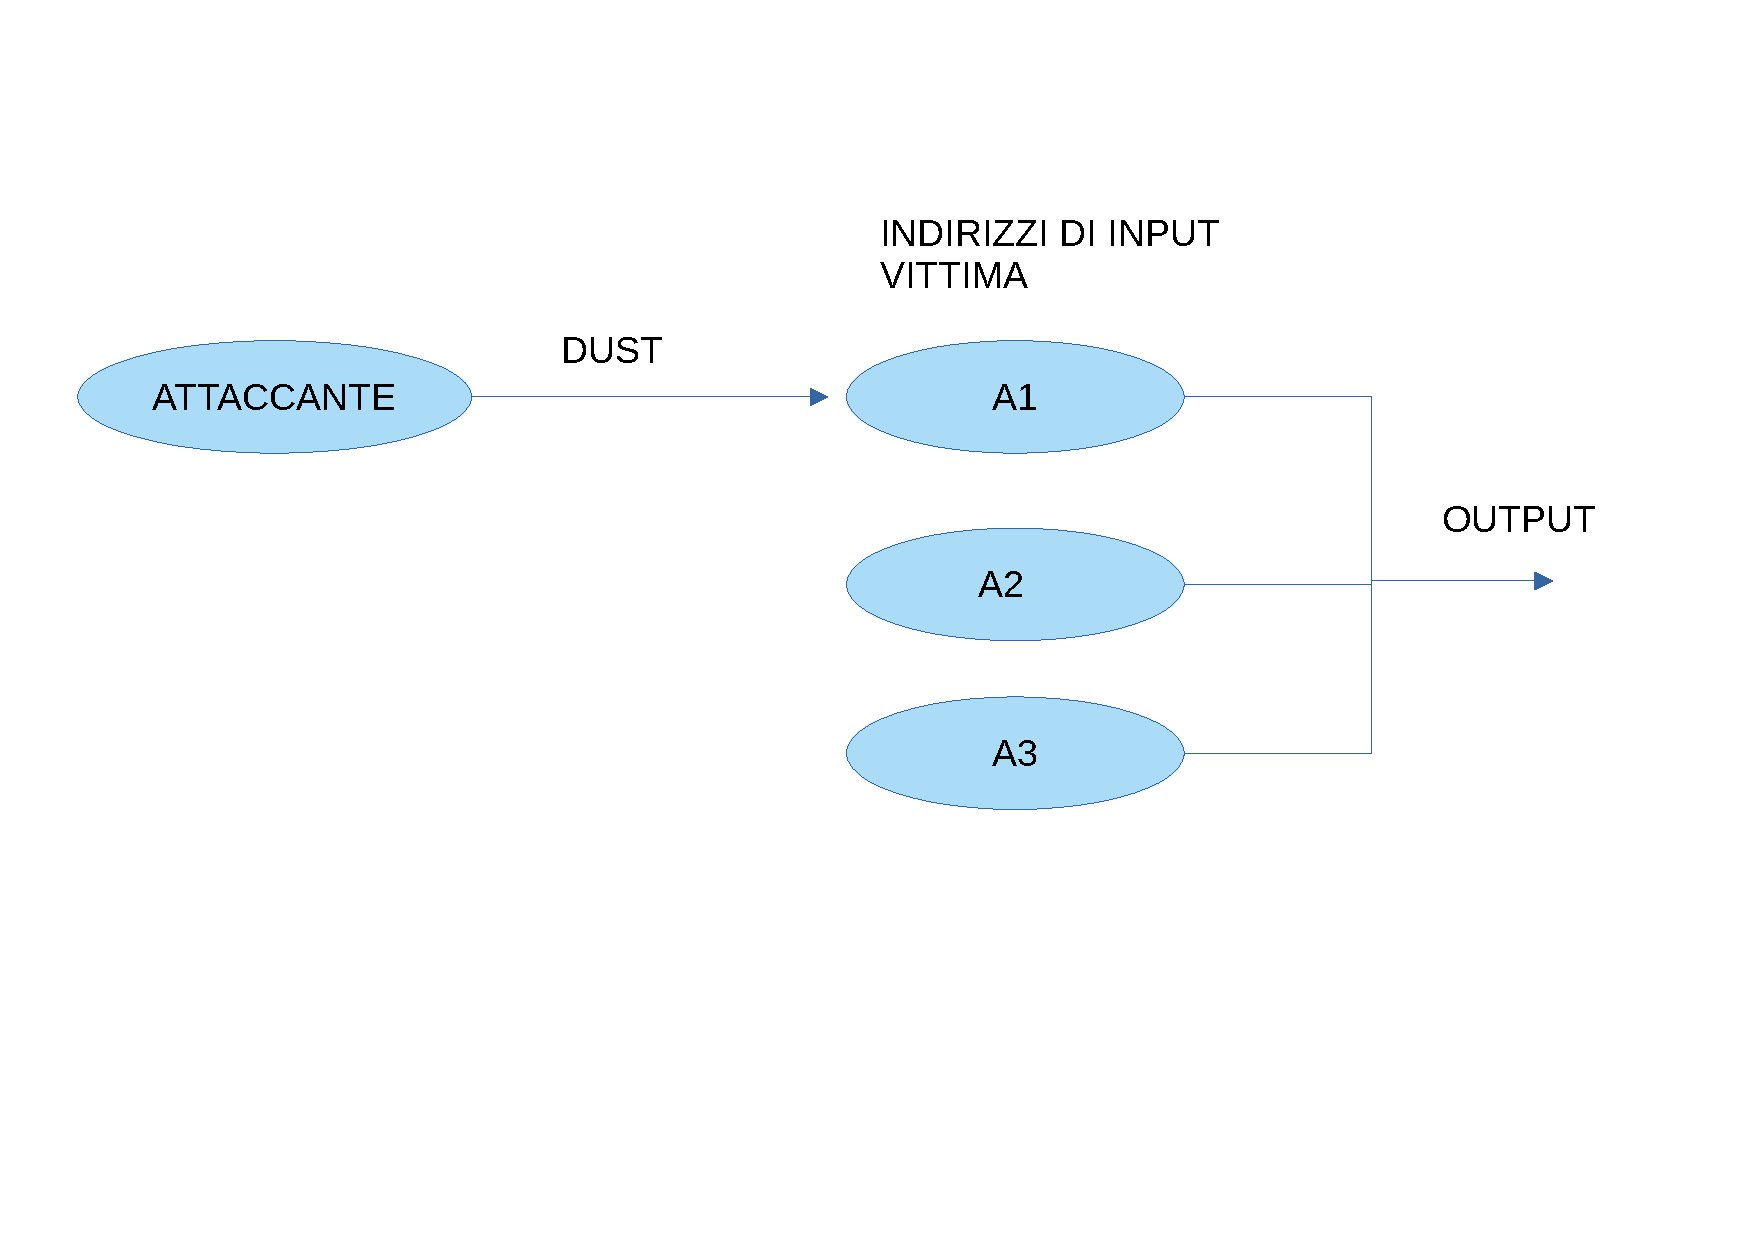
\includegraphics[scale=0.3]{Images/successo.pdf}
    \caption{Schema Attacco di Successo}
    \label{fig:success}
\end{figure}
\FloatBarrier
Nel secondo caso invece l'importo è stato speso in una transazione dove sono presenti più input ma tutti legati allo stesso address. In questa situazione l'attaccante non collega address diversi e quindi fallisce nel tentativo di de-anonimizzazione. Questa situazione è visibile nella figura \ref{fig:fallito}. 
\begin{figure}[h!]
    \centering
    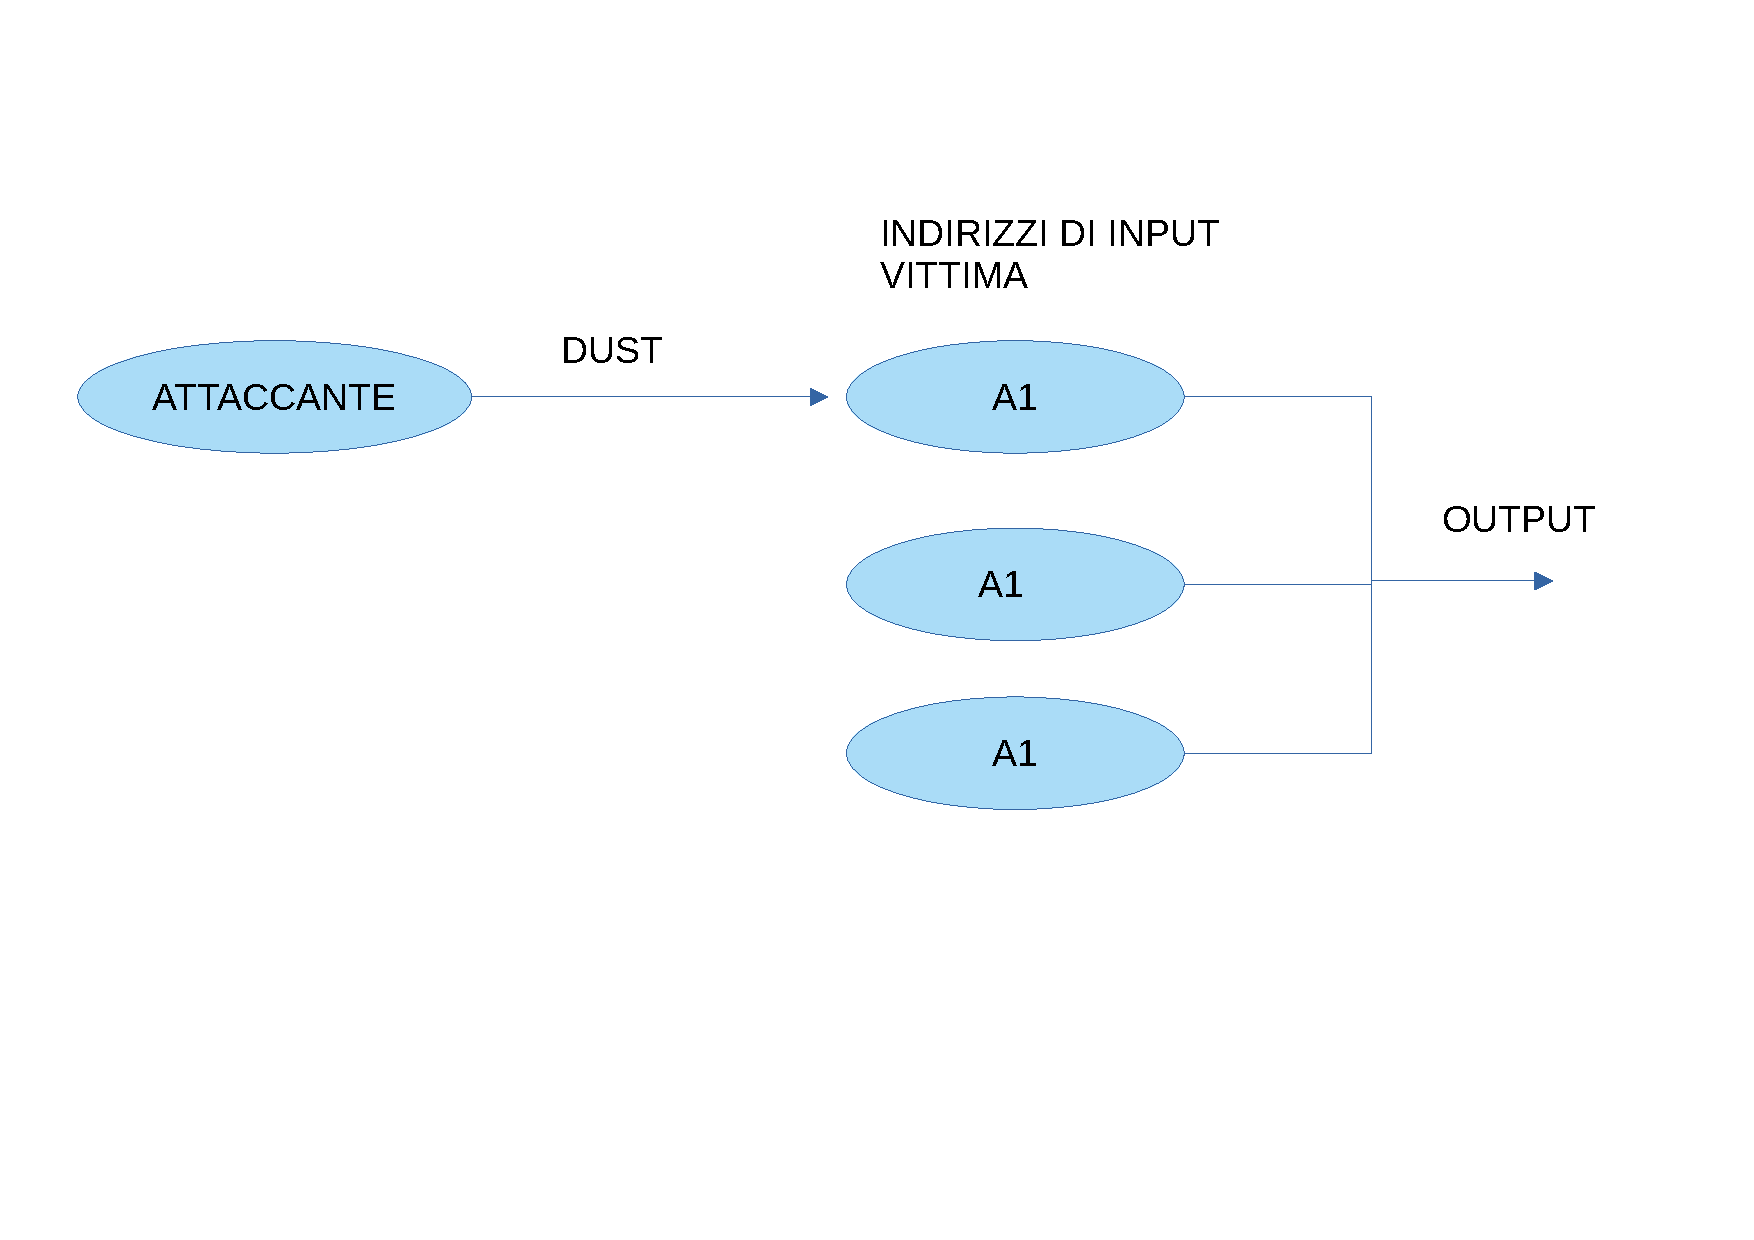
\includegraphics[scale=0.35]{Images/fallimento.pdf}
    \caption{Schema Attacco Fallito}
    \label{fig:fallito}
\end{figure}
\FloatBarrier
Il \textit{dust attack} quindi risulta più efficace soprattutto contro gli address che hanno un bilancio complessivo pari a zero proprio perché obbliga la vittima a spendere la cifra ottenuta con altri suoi address diversi.\\\\
Terzo e ultimo caso semplicemente la vittima non spende il dust ricevuto troncando l'attacco sul nascere.\\\\
È importante notrare che il dust attack non permette di rubare fondi di altri utenti né permette di scoprire le informazioni personali, per esempio nome e cognome, della vittima ma permette di ricavare un'importante informazione che può essere usata in seguito per effettuare attacchi più pericolosi.
\section{Conseguenze}
Come detto in precedenza questa tipo di de-anonimizzazione di per sé non costituisce un problema. Può diventarlo se viene usata come mezzo per altri tipi di attacchi. In generale il Dust Attack non per forza è legato a phishing o estorsioni ma potrebbe essere usato dalle autorità per tenere traccia degli utenti ed eventualmente rilevare attività illegali. Infatti una volta otteuto un cluster di address riesco a tracciare l'attività di un singolo utente e non più di un singolo address. Le autorità potrebbero notare che certi utenti interagiscono con address legati a mercati neri, e quindi indagare ulteriormente per scoprire l'identità di queste persone. Uno dei punti fondamentali è legare informazioni personali, come e-mail, nome ed altro, a address Bitcoin. In molti casi sono gli utenti stessi che pubblicano sui forum i loro address, in altre situazioni invece è possibile sfruttare gli exchange come Coinbase.\\\\Gli exchange sono servizi che permettono lo scambio tra criptovalute e valute tradizionali basandosi sul valore di mercato della criptovaluta. In exchange come Coinbase è necessario creare un account fornendo informazioni personali come nome, cognome, email ed altro e, una volta registrati, viene creato un wallet associato a quel particolare account. Siccome gli exchange sono esposti ad attacchi hacker molti utenti trasferiscono i loro bitcoin su address appartenenti a software wallet, per esempio Wasabi Wallet.\\\\
Una volta che un utente effettua un deposito dal wallet, vittima di Dust Attack, ad un account exchange ecco che l'attaccante collega gli address al proprietario. Una volta ottenuta l'identità del proprietario l'attaccante può eseguire elaborati attacchi di phishing oppure può estorcergli il denaro minacciandolo di rivelare a tutti l'informazione ottenuta.\\ Il Dust Attack però non risulta particolarmente difficile da contrastare, nel paragrafo successivo verranno mostrati due metodi per difendersi da questo tipo di attacco.
\section{Contromisure}
Due metodi per contrastare il dust attack sono:
    \begin{enumerate}
        \item non spendere l'importo dust ricevuto; 
        \item utlizzare servizi di "dust collecting". 
    \end{enumerate}
La prima soluzione, semplice ed efficace, permette di troncare l'attacco sul nascere. Infatti se il dust non viene speso l'attaccante non potrà mai collegare address diversi dello stesso utente. 
Questo metodo può esserre effettuato in diversi software wallet; per esempio Samurai Wallet \footnote{fonte:\url{https://twitter.com/samouraiwallet/status/1055345822076936192?lang=en}}, nel 2018, consigliò ai suoi utenti, possibili vittime di dust attack,  di contrassegnare come "do not spend" l'output dust ricevuto.\\\\
La seconda soluzione riguarda i servizi di "dust collecting", per esempio Dust-B-Gone \cite{Dbg}.
L'obiettivo di questo meccanismo è di impedire la de-anonimizzazione tramite la generazione di una singola transazione dove gli input dust provengono da utenti diversi. L'importo complessivo viene trasformato in fee per i miners. \\Poichè gli address di input appartengono a utenti differenti, l'attaccante fallisce nel tentativo di de-anonimizzazione.